% Options for packages loaded elsewhere
\PassOptionsToPackage{unicode}{hyperref}
\PassOptionsToPackage{hyphens}{url}
%
\documentclass[
  english,
  jou,floatsintext]{apa6}
\usepackage{amsmath,amssymb}
\usepackage{lmodern}
\usepackage{ifxetex,ifluatex}
\ifnum 0\ifxetex 1\fi\ifluatex 1\fi=0 % if pdftex
  \usepackage[T1]{fontenc}
  \usepackage[utf8]{inputenc}
  \usepackage{textcomp} % provide euro and other symbols
\else % if luatex or xetex
  \usepackage{unicode-math}
  \defaultfontfeatures{Scale=MatchLowercase}
  \defaultfontfeatures[\rmfamily]{Ligatures=TeX,Scale=1}
\fi
% Use upquote if available, for straight quotes in verbatim environments
\IfFileExists{upquote.sty}{\usepackage{upquote}}{}
\IfFileExists{microtype.sty}{% use microtype if available
  \usepackage[]{microtype}
  \UseMicrotypeSet[protrusion]{basicmath} % disable protrusion for tt fonts
}{}
\makeatletter
\@ifundefined{KOMAClassName}{% if non-KOMA class
  \IfFileExists{parskip.sty}{%
    \usepackage{parskip}
  }{% else
    \setlength{\parindent}{0pt}
    \setlength{\parskip}{6pt plus 2pt minus 1pt}}
}{% if KOMA class
  \KOMAoptions{parskip=half}}
\makeatother
\usepackage{xcolor}
\IfFileExists{xurl.sty}{\usepackage{xurl}}{} % add URL line breaks if available
\IfFileExists{bookmark.sty}{\usepackage{bookmark}}{\usepackage{hyperref}}
\hypersetup{
  pdftitle={Unveiling the Structure of Heart Rate Variability (HRV) Indices: A Data-driven Meta-clustering Approach},
  pdfauthor={Tam Pham1, Zen J. Lau1, S.H. Annabel Chen1, 2, 3, 4, *, \& Dominique Makowski1, *},
  pdflang={en-EN},
  pdfkeywords={HRV, ECG, Clustering},
  hidelinks,
  pdfcreator={LaTeX via pandoc}}
\urlstyle{same} % disable monospaced font for URLs
\usepackage{graphicx}
\makeatletter
\def\maxwidth{\ifdim\Gin@nat@width>\linewidth\linewidth\else\Gin@nat@width\fi}
\def\maxheight{\ifdim\Gin@nat@height>\textheight\textheight\else\Gin@nat@height\fi}
\makeatother
% Scale images if necessary, so that they will not overflow the page
% margins by default, and it is still possible to overwrite the defaults
% using explicit options in \includegraphics[width, height, ...]{}
\setkeys{Gin}{width=\maxwidth,height=\maxheight,keepaspectratio}
% Set default figure placement to htbp
\makeatletter
\def\fps@figure{htbp}
\makeatother
\setlength{\emergencystretch}{3em} % prevent overfull lines
\providecommand{\tightlist}{%
  \setlength{\itemsep}{0pt}\setlength{\parskip}{0pt}}
\setcounter{secnumdepth}{-\maxdimen} % remove section numbering
% Make \paragraph and \subparagraph free-standing
\ifx\paragraph\undefined\else
  \let\oldparagraph\paragraph
  \renewcommand{\paragraph}[1]{\oldparagraph{#1}\mbox{}}
\fi
\ifx\subparagraph\undefined\else
  \let\oldsubparagraph\subparagraph
  \renewcommand{\subparagraph}[1]{\oldsubparagraph{#1}\mbox{}}
\fi
% Manuscript styling
\usepackage{upgreek}
\captionsetup{font=singlespacing,justification=justified}

% Table formatting
\usepackage{longtable}
\usepackage{lscape}
% \usepackage[counterclockwise]{rotating}   % Landscape page setup for large tables
\usepackage{multirow}		% Table styling
\usepackage{tabularx}		% Control Column width
\usepackage[flushleft]{threeparttable}	% Allows for three part tables with a specified notes section
\usepackage{threeparttablex}            % Lets threeparttable work with longtable

% Create new environments so endfloat can handle them
% \newenvironment{ltable}
%   {\begin{landscape}\begin{center}\begin{threeparttable}}
%   {\end{threeparttable}\end{center}\end{landscape}}
\newenvironment{lltable}{\begin{landscape}\begin{center}\begin{ThreePartTable}}{\end{ThreePartTable}\end{center}\end{landscape}}

% Enables adjusting longtable caption width to table width
% Solution found at http://golatex.de/longtable-mit-caption-so-breit-wie-die-tabelle-t15767.html
\makeatletter
\newcommand\LastLTentrywidth{1em}
\newlength\longtablewidth
\setlength{\longtablewidth}{1in}
\newcommand{\getlongtablewidth}{\begingroup \ifcsname LT@\roman{LT@tables}\endcsname \global\longtablewidth=0pt \renewcommand{\LT@entry}[2]{\global\advance\longtablewidth by ##2\relax\gdef\LastLTentrywidth{##2}}\@nameuse{LT@\roman{LT@tables}} \fi \endgroup}

% \setlength{\parindent}{0.5in}
% \setlength{\parskip}{0pt plus 0pt minus 0pt}

% \usepackage{etoolbox}
\makeatletter
\patchcmd{\HyOrg@maketitle}
  {\section{\normalfont\normalsize\abstractname}}
  {\section*{\normalfont\normalsize\abstractname}}
  {}{\typeout{Failed to patch abstract.}}
\patchcmd{\HyOrg@maketitle}
  {\section{\protect\normalfont{\@title}}}
  {\section*{\protect\normalfont{\@title}}}
  {}{\typeout{Failed to patch title.}}
\makeatother
\shorttitle{Structure of HRV indices}
\keywords{HRV, ECG, Clustering\newline\indent Word count: 4287}
\usepackage{dblfloatfix}


\usepackage{lineno}

\linenumbers
\usepackage{csquotes}
\usepackage[labelfont=bf, font={color=gray,small}]{caption}
\usepackage{float}
\usepackage[document]{ragged2e}
\usepackage{booktabs}
\usepackage{makecell}
\ifxetex
  % Load polyglossia as late as possible: uses bidi with RTL langages (e.g. Hebrew, Arabic)
  \usepackage{polyglossia}
  \setmainlanguage[]{english}
\else
  \usepackage[main=english]{babel}
% get rid of language-specific shorthands (see #6817):
\let\LanguageShortHands\languageshorthands
\def\languageshorthands#1{}
\fi
\ifluatex
  \usepackage{selnolig}  % disable illegal ligatures
\fi
\newlength{\cslhangindent}
\setlength{\cslhangindent}{1.5em}
\newlength{\csllabelwidth}
\setlength{\csllabelwidth}{3em}
\newenvironment{CSLReferences}[2] % #1 hanging-ident, #2 entry spacing
 {% don't indent paragraphs
  \setlength{\parindent}{0pt}
  % turn on hanging indent if param 1 is 1
  \ifodd #1 \everypar{\setlength{\hangindent}{\cslhangindent}}\ignorespaces\fi
  % set entry spacing
  \ifnum #2 > 0
  \setlength{\parskip}{#2\baselineskip}
  \fi
 }%
 {}
\usepackage{calc}
\newcommand{\CSLBlock}[1]{#1\hfill\break}
\newcommand{\CSLLeftMargin}[1]{\parbox[t]{\csllabelwidth}{#1}}
\newcommand{\CSLRightInline}[1]{\parbox[t]{\linewidth - \csllabelwidth}{#1}\break}
\newcommand{\CSLIndent}[1]{\hspace{\cslhangindent}#1}

\title{\textbf{Unveiling the Structure of Heart Rate Variability (HRV) Indices: A Data-driven Meta-clustering Approach}}
\author{Tam Pham\textsuperscript{1}, Zen J. Lau\textsuperscript{1}, S.H. Annabel Chen\textsuperscript{1, 2, 3, 4, *}, \& Dominique Makowski\textsuperscript{1, *}}
\date{}


\authornote{

Correspondence concerning this article should be addressed to S.H. Annabel Chen, HSS 04-19, 48 Nanyang Avenue, Singapore. E-mail: \href{mailto:annabelchen@ntu.edu.sg}{\nolinkurl{annabelchen@ntu.edu.sg}}

}

\affiliation{\vspace{0.5cm}\textsuperscript{1} School of Social Sciences, Nanyang Technological University, Singapore\\\textsuperscript{2} Centre for Research and Development in Learning, Nanyang Technological University, Singapore\\\textsuperscript{3} Lee Kong Chian School of Medicine, Nanyang Technological University, Singapore\\\textsuperscript{4} National Institute of Education, Nanyang Technological University, Singapore}

\abstract{
Heart Rate Variability (HRV) can be estimated using a myriad of mathematical indices, but the lack of systematic comparison between these indices renders the evaluation and interpretation of results difficult. In this study, we assessed the relationship between 57 HRV metrics collected from 302 human recordings using a variety of structure-analysis algorithms. We then applied a meta-clustering approach to combine their results and obtain a robust and reliable view of the observed relationships. We found that HRV metrics can be clustered into main 3 groups, representing the distribution-related features, harmony-related features, and frequency/complexity features. We describe and discuss their substructures and derive recommendations on which indices to prioritize for parsimonious, yet comprehensive HRV-related data analysis and reporting.
}



\begin{document}
\maketitle

\justify

Heart Rate Variability (HRV), reflecting the heart's ability to effectively regulate and adapt to internal and external environmental changes, has been linked to many physical and mental health outcomes (e.g., cardiac complications, Laitio et al., 2007; diabetes, Kudat et al., 2006; mood disorders, Bassett, 2016; cognitive functioning, Forte et al., 2019). The various indices used in the assessment of HRV are broadly categorized based on their mathematical underpinnings, with categories conventionally including the \emph{time-domain}, \emph{frequency-domain}, and \emph{nonlinear dynamics}.

Time-domain indices are overall the simplest and most straightforward method of quantifying the variability of normal (i.e., excluding abnormal beats such as ectopic beats) heartbeat intervals (NN intervals - NNIs). Some commonly derived indices include the standard deviation of all NN intervals (\emph{SDNN}), the root mean square of the sum of successive differences of NN intervals (\emph{RMSSD}), and the percentage of adjacent NN intervals separated by more than 50ms (\emph{pNN50}). While time-domain methods offer computational ease, they are less sensitive in distinguishing between the contributions of sympathetic and parasympathetic branches (Acharya et al., 2006). Frequency-domain indices, on the other hand, target the assessment of these different regulatory mechanisms by investigating how the HRV power spectrum distributes across different frequency bands (e.g, low frequency, \emph{LF} or high frequency, \emph{HF}). Other indices that fall under the frequency domain include derivatives of the aforementioned components, such as the ratio of \emph{LF} to \emph{HF} (\emph{LF/HF}) power and their normalized (e.g., \emph{LFn}, \emph{HFn}) and natural logarithmic variants (e.g., \emph{LnHF}). Finally, drawn from concepts of non-linear dynamics and chaos theory (Golberger, 1996; Lau et al., 2021), non-linear indices were introduced to better characterize the complex physiological mechanisms underlying HRV. Prominent indices include measures obtained from a Poincaré plot where an ellipse is fitted to a scatterplot of each NN interval against its preceding one (e.g., the standard deviation of the short-term, \emph{SD1} and long-term, \emph{SD2} NN interval variability, as well as its corresponding ratio, \emph{SD1/SD2}, Brennan et al., 2001). Other non-linear indices that fall under this category, such as Detrended Fluctuation Analysis (\emph{DFA}), multi-fractal \emph{DFA} (\emph{MF-DFA}) and correlation dimension (\emph{CD}), account for the fractal properties of HRV, while entropy measures like approximate entropy (\emph{ApEn}), sample entropy (\emph{SampEn}), and multiscale entropy (\emph{MSE}) quantify the amount of regularity in the heart rate (HR) time series (Voss et al., 2009). However, new methods are continually being developed, including time-frequency domain analysis (Faust et al., 2004) and HR fragmentation (Costa et al., 2017). For a more comprehensive description of all HRV indices, see Pham et al. (2021).

In light of the popularity of HRV analysis for investigating health and disease, the multitude of existing metrics warrants some concerns. Firstly, the functional association of these indices with physiological mechanisms is poorly understood (Fatisson et al., 2016; Hayano \& Yuda, 2019), with the indices often used interchangeably to describe HRV as a general concept. This not only makes it difficult to interpret and report the complex patterns of (sometimes inconsistent) results but can also aggravate replicability issues, as different studies, when examining the same phenomenon (e.g., cognitive flexibility, aging), might rely on different indices to describe the relationships with HRV. Apart from this conceptual hurdle pertaining to the unclear relationship between the mathematical indices and their physiological meaning, another pragmatic issue lies in the shared similarities and overlaps between many of these metrics. For instance, early studies have investigated the relationships between time-domain and frequency-domain indices, showing that not only were \emph{RMSSD} and \emph{pNN50} strongly correlated with each other (above 0.9, Bigger Jr et al., 1989), they were also highly associated with \emph{HF} power (Bigger Jr et al., 1989; Kleiger et al., 2005; Otzenberger et al., 1998), suggesting that these measures could be treated as surrogates for each other in assessing the parasympathetic modulation of HRV. This observation is warranted given that the former is computed from the differences across consecutive NN intervals, and hence, they reflect mainly high-frequency oscillatory patterns in HR and are independent of long-term changes. On the other hand, \emph{SDNN}, which has been thought to reflect both sympathetic and parasympathetic activity, is correlated to total power in the HRV power spectrum (Bigger Jr et al., 1989). Recent years also witnessed the emergence of debates regarding the traditional conceptualization of \emph{SD1} and \emph{SD2} as non-linear indices, particularly when Ciccone et al. (2017) pointed out that \emph{RMSSD} and \emph{SD1} are actually mathematically equivalent. Consequently, studies that report both of these short-term HRV indices often independently arrive at identical statistical results without addressing this equivalence (Leite et al., 2015; Peng et al., 2015; Rossi et al., 2015). Additionally, other studies have also drawn similarities between \emph{SD1/SD2} and \emph{LF/HF} in their indexing of the balance between short- and long-term HRV (Brennan et al., 2002; Guzik et al., 2007). These overlaps, if not taken into account in analyses, can lead to statistical issues, such as inflated confidence in the results (shown by an artificially high number of indices appearing to agree with a given trend), collinearity issues (if multiple indices are jointly used as predictors), potential over-correction (e.g., for Bonferroni-type p-value adjustment methods), and needlessly complex and cluttered patterns of results (Dormann et al., 2013; Mela \& Kopalle, 2002; Næs \& Mevik, 2001).

The aim of this study is thus to increase the understanding of the relationships between HRV indices using a data-driven approach. Beyond simply computing and reporting the correlations between the indices, the goal is to assess the presence of groups (i.e., clusters) of metrics, subsequently describe them, and discuss hypotheses as to their existence. While there exist different approaches to assign data to different groups based on their level of associations (see Nguyen Phuc Thu et al., 2019), there is no gold standard or clear guidelines to determine the most appropriate method for grouping these physiological indices. As such, choosing one method and presenting its solution as a definitive one can be misleading. Thus, we will explore the structure of HRV indices using a consensus-based methodology (Bhattacharjee et al., 2001; Kuncheva, 2014; Monti et al., 2003), henceforth referred to as \emph{meta-clustering}, where the results of multiple structure analysis approaches are systematically combined to highlight the most robust associations between HRV indices. To the best of our knowledge, this is the first attempt to apply the consensus-based framework to the clustering of an extensive list of the most common and up-to-date HRV indices.

\hypertarget{methods}{%
\section{Methods}\label{methods}}

The electrocardiogram (ECG) data of 302 participants were extracted from 6 open-access databases described below. The script to download and format the databases are available at \url{https://github.com/neuropsychology/NeuroKit/tree/master/data}. The processed data, as well as the full reproducible analysis script, including additional descriptions of each approach and the solutions of each individual clustering method, are available at this GitHub repository (\url{https://github.com/Tam-Pham/HRVStructure}).

\hypertarget{databases}{%
\subsection{Databases}\label{databases}}

The Glasgow University Database (GUDB) database (Howell \& Porr, 2018) contains ECG recordings from 25 healthy participants (\textgreater{} 18 years old) performing five different two-minute tasks (sitting, doing a maths test on a tablet, walking on a treadmill, running on a treadmill, using a handbike). All recordings were sampled at 250 Hz.

The MIT-BIH Arrhythmia Database (MIT-Arrhythmia and MIT-Arrhythmia-x) database (Moody \& Mark, 2001) contains 48 ECG recordings (25 men, 32-89 years old; 22 women, 23-89 years old) from a mixed population of patients. All recordings were sampled at 360 Hz and lasted for 30 minutes.

The Fantasia database (Iyengar et al., 1996) contains ECG recordings from 20 young (21-34 years old) and 20 elderly (68-85 years old) healthy participants. All participants remained in a resting state in sinus rhythm while watching the movie Fantasia (Disney, 1940) that helped to maintain wakefulness. All recordings were sampled at 250 Hz and lasted for 120 minutes.

The MIT-BIH Normal Sinus Rhythm Database (MIT-Normal) database (Goldberger et al., 2000) contains long-term (\(\approx\) 24h) ECG recordings from 18 participants (5 men, 26-45 years old; 13 women, 20-50 years old). All recordings were sampled at 128 Hz and due to memory limits, we kept only the second and third hours of each recording (with the loose assumption that the first hour might be less representative of the rest of the recording and a duration of 120 minutes would match those from the Fantasia database).

The MIT-BIH Long-term ECG Database (MIT-Long-term) database (Goldberger et al., 2000) contains long-term (14 to 22 hours each) ECG recordings from 7 participants (6 men, 46-88 years old; 1 woman, 71 years old). All recordings were sampled at 128 Hz and due to memory limits, we kept only the second and third hours of each recording.

The last dataset came from resting-state recordings of the authors' other empirical studies (\url{https://github.com/neuropsychology/RestingState}). This dataset contains ECG recordings sampled at 4000 Hz from 43 healthy participants (\textgreater{} 18 years old) that underwent 8 minutes of eyes-closed, seated position, resting state.

\hypertarget{data-analysis}{%
\subsection{Data Analysis}\label{data-analysis}}

The \texttt{NeuroKit2} software (Makowski et al., 2021) was used to preprocess the raw ECG signals (when available), locate R-peaks and subsequently, compute all the HRV indices (see \textbf{Table 1} for the abbreviations and description of all HRV indices). The rest of the data analysis was carried out with R (R Core Team, 2019) and the \emph{easystats} ecosystem (Ludecke et al., 2019; Lüdecke, Patil, et al., 2021; Makowski et al., 2019, 2020). Reproducible scripts are available at \url{https://github.com/Tam-Pham/HRVStructure}.

We started by identifying indices that were near-perfect duplicates (\textbar r\textbar{} \textgreater{} 0.999) and removed them (to prevent further statistical issues such as positive definite correlation matrices). For each index, we then removed extreme observations (\textgreater{} .9999 percentile of the median absolute deviation from the median) - \(\approx\) 4\% of data - using the \texttt{check\_outliers} function in the \emph{performance} R package (Lüdecke, Ben-Shachar, et al., 2021). On average, 5.61\% of data was detected as outliers and removed. Multiple structural methods were then applied to analyze the associations between the HRV indices, such as dimensionality analyses (including Principal Component Analysis - PCA, and Exploratory Factor Analysis - EFA), clustering (including k-means, k-medoids, hierarchical clustering, DBSCAN, HBSCAN, mixture model algorithms), as well as network-based approaches (exploratory graph analysis; EGA). While the individual solutions are described in the Supplementary Materials, the study aimed to aggregate them to identify the robust groups identified across these methods.

The \emph{meta-clustering} approach (Lüdecke et al., 2020; which finds echoes in \emph{consensus clustering}; see Monti et al., 2003) treats the unique clustering solutions as an ensemble, from which a probability matrix is derived (see \textbf{Figure 1}). This matrix contains, for each pair of HRV indices, the probability of being grouped together. For instance, if two indices have been assigned to a similar cluster by 5 out of 10 clustering methods, then the probability associated with this pair is 0.5. This probability matrix is then treated as a distance matrix and submitted to hierarchical clustering. Essentially, this approach is based on the notion that, as each clustering algorithm embodies a different angle in which it sees the data, cross-validating the phenomenon of interest using different perspectives leads to more accurate results.

\hypertarget{results}{%
\section{Results}\label{results}}

Indices that were identified as redundant in the correlation analysis, and subsequently removed, included 1) \emph{SDSD}, \emph{SD1}, \emph{SD1a} and \emph{SD1d} (duplicates of RMSSD); 2) \emph{SDNNa} and \emph{SDNNd} (duplicates of \emph{SDNN}); 3) \emph{SD2a} and \emph{SD2d} (duplicates of \emph{SD2}); 4) \emph{Cd} (duplicate of \emph{Ca}); 5) \emph{C1d} (duplicate of \emph{C1a}); and 6) \emph{C2d} (duplicate of \emph{C2a}). The indices that were kept were selected based on their higher popularity (e.g., \emph{RMSSD}) or functional meaning (e.g., acceleration for \emph{Ca}).

PCA solutions with 9 and 12 components were deemed suitable (see the \texttt{n\_components} function in the \emph{parameters} package, Lüdecke et al., 2020) and extracted, and each component was treated as a cluster containing indices with the highest loadings. Following a similar optimizing procedure, two solutions of 9 factors and 12 factors were extracted using EFA. See \textbf{Tables 1-4} in \emph{Supplementary Material} for the item loadings of dimension solutions.

Three optimal structure solutions of 2-cluster, 7-cluster, and 10-cluster were identified for k-means clustering (see the \texttt{n\_clusters} function in the \emph{parameters} package) and a 3-cluster solution was extracted for k-medoids clustering (see \texttt{pamk} function, Hennig \& Imports, 2015). Two hierarchical clustering models were also constructed using Euclidean distance method and average linkage method. These bootstrapping-based solutions to cluster selection with a confidence level of 90\% and 95\% identified 13 and 11 significant clusters respectively (see Suzuki \& Shimodaira, 2006). Other unsupervised clustering approaches, DBSCAN and HDBSCAN, suggested two additional structure solutions of respectively 6 and 15 clusters, and the mixture model yielded a solution of 6 clusters. See \textbf{Figures 1-9} in \emph{Supplementary Material} for the clustergrams/ deprograms results of clustering solutions.

Finally, two solutions were extracted from the network-based EGA approach using two network estimation algorithms, \emph{GLASSO} and \emph{TMFG}, in combination with the \emph{louvian} network community detection algorithm (H. Golino et al., 2020; H. F. Golino \& Epskamp, 2017). The two networks were associated with structure solutions of 7 and 6 clusters respectively. See \textbf{Figures 10-11} in \emph{Supplementary Material} for the results of network solutions.

Using the fifteen structure solutions from the aforementioned methods, we computed the probability matrix representing each pair of HRV indices being assigned to the same cluster (see \textbf{Figure 1}). The matrix was inverted to form a distance matrix and submitted to hierarchical cluster analysis with average linkage method. The results of the \emph{meta-clustering} approach are presented in \textbf{Figure 2}. The most closely related clusters of indices include the cluster of time-domain indices (e.g., \emph{RMSSD}, \emph{pNN50}, \emph{SDNN}, \emph{MadNN}), the cluster of heart rate asymmetry indices (\emph{HRA}; e.g., \emph{PAS}, \emph{PSS}, \emph{PIP}), the cluster of heart rate fragmentation indices (\emph{HRF}; e.g., \emph{PI}, \emph{GI}, \emph{AI}), and the cluster of \emph{DFA} indices with the low-frequency indices (e.g., \emph{LFHF}, \emph{LFn}). The remaining indices, which include the high-frequency indices (e.g., \emph{HF}, \emph{HFn}) and the different non-linear indices (e.g., \emph{CD}, \emph{LZC}, \emph{SampEn}, \emph{FuzzyEn}) were relatively closely related to each other in the final structure. The cluster memberships (Level 2 in \textbf{Table 1}) were determined by a vertical height cut at 0.8 and within each cluster, the center was identified as the average value of all members. The relative distances from the center, representing the members' centrality values or degree of cluster representativeness, were calculated and summarized in \textbf{Table 1}.

\begin{figure}

{\centering 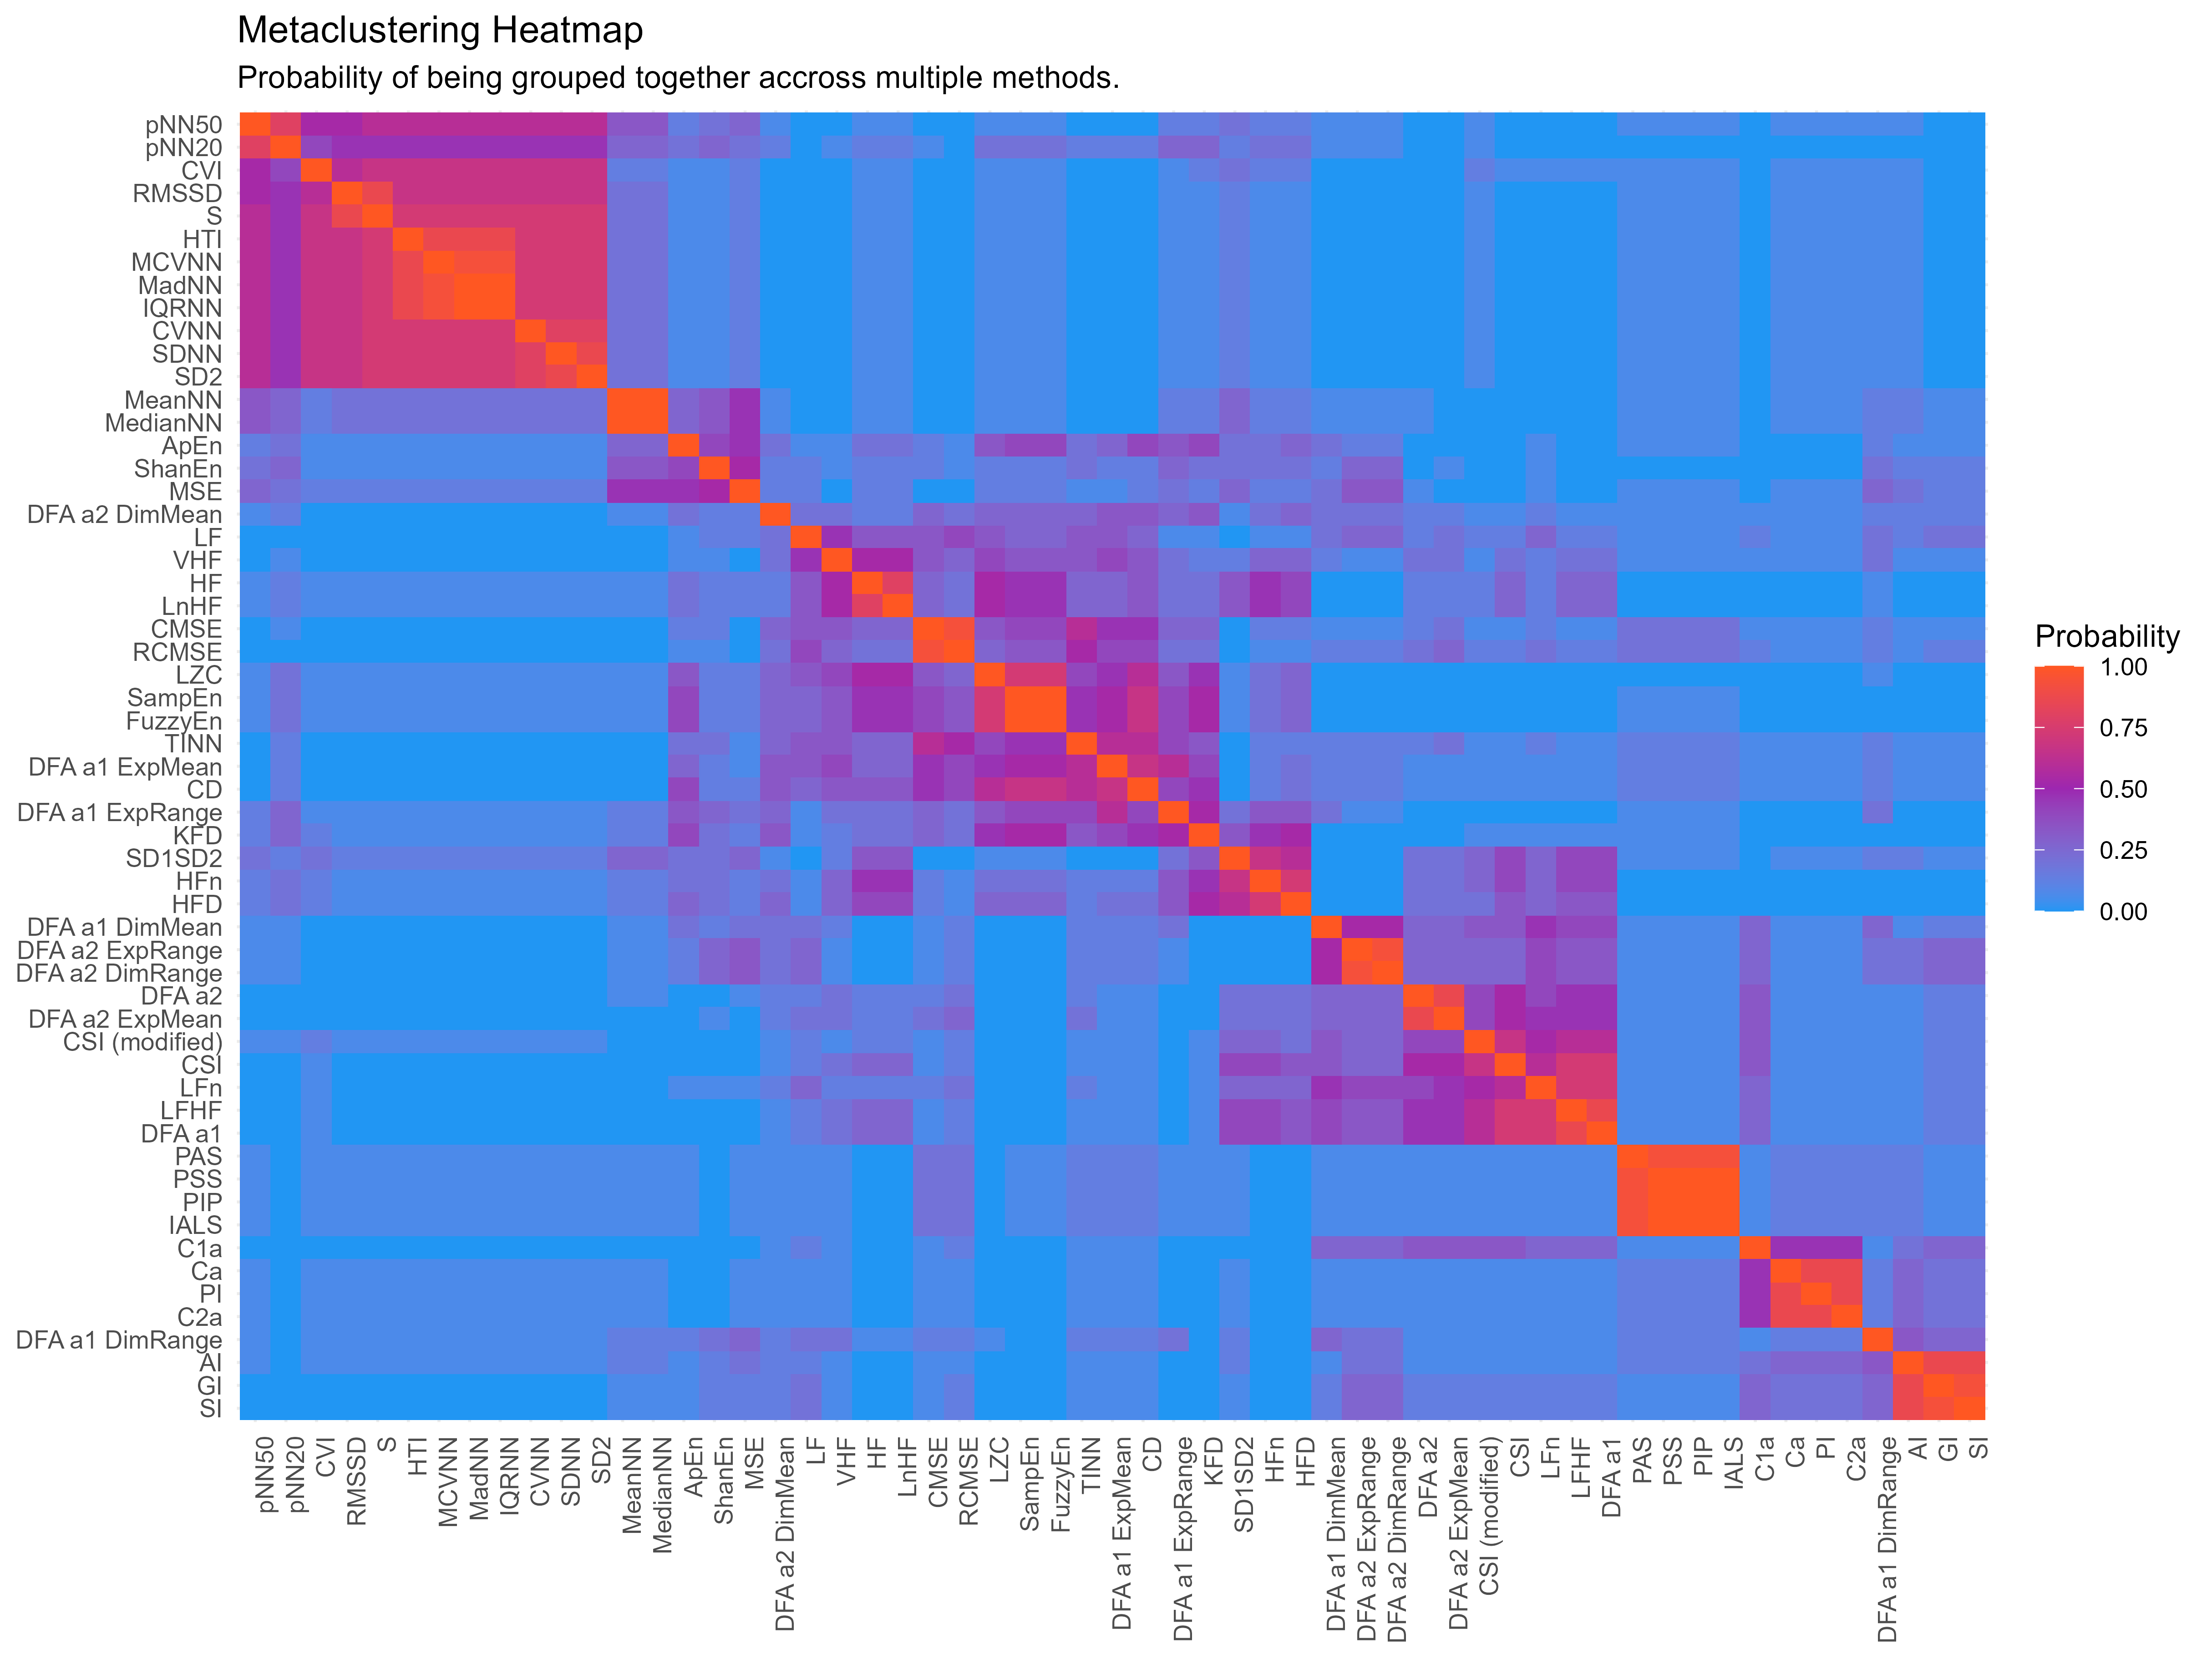
\includegraphics[width=0.5\textwidth]{figures/figure_probability_matrix} 

}

\caption{Probability Matrix that represents the probability of each pair of HRV indices being assigned to the same cluster. The probability can take any value from 0, which indicates that no solution assigned the two indices to the same cluster, to 1, which indicates that all solutions suggested the two indices belong to the same group. The absolute proximity of every variable with itself is represented by the main diagonal in red (probability = 1). From the heatmap, we can see a clear structure of 6 clusters, corresponding to the Level 2 groupings in Table 1, emerged. As compared to the other clusters, the two big clusters in the centre of the heatmap, "absolute" and "relative", are less clear.}\label{fig:Figure1}
\end{figure}

\hypertarget{discussion}{%
\section{Discussion}\label{discussion}}

In this study, we applied various structure analysis techniques to explore the relationships between HRV indices. By combining the domain knowledge from a multitude of statistical methods, the meta-clustering approach maximizes the stability of the final HRV structure and circumvents the lack of objective criteria for the selection of techniques. The meta-clustering solution presented in \textbf{Figure 2} yielded an intriguing and complex pattern of associations and groupings, with three overarching clusters observed at the top level (Level 1 in \textbf{Table 1}) that we will now describe and discuss.

\begin{figure}

{\centering 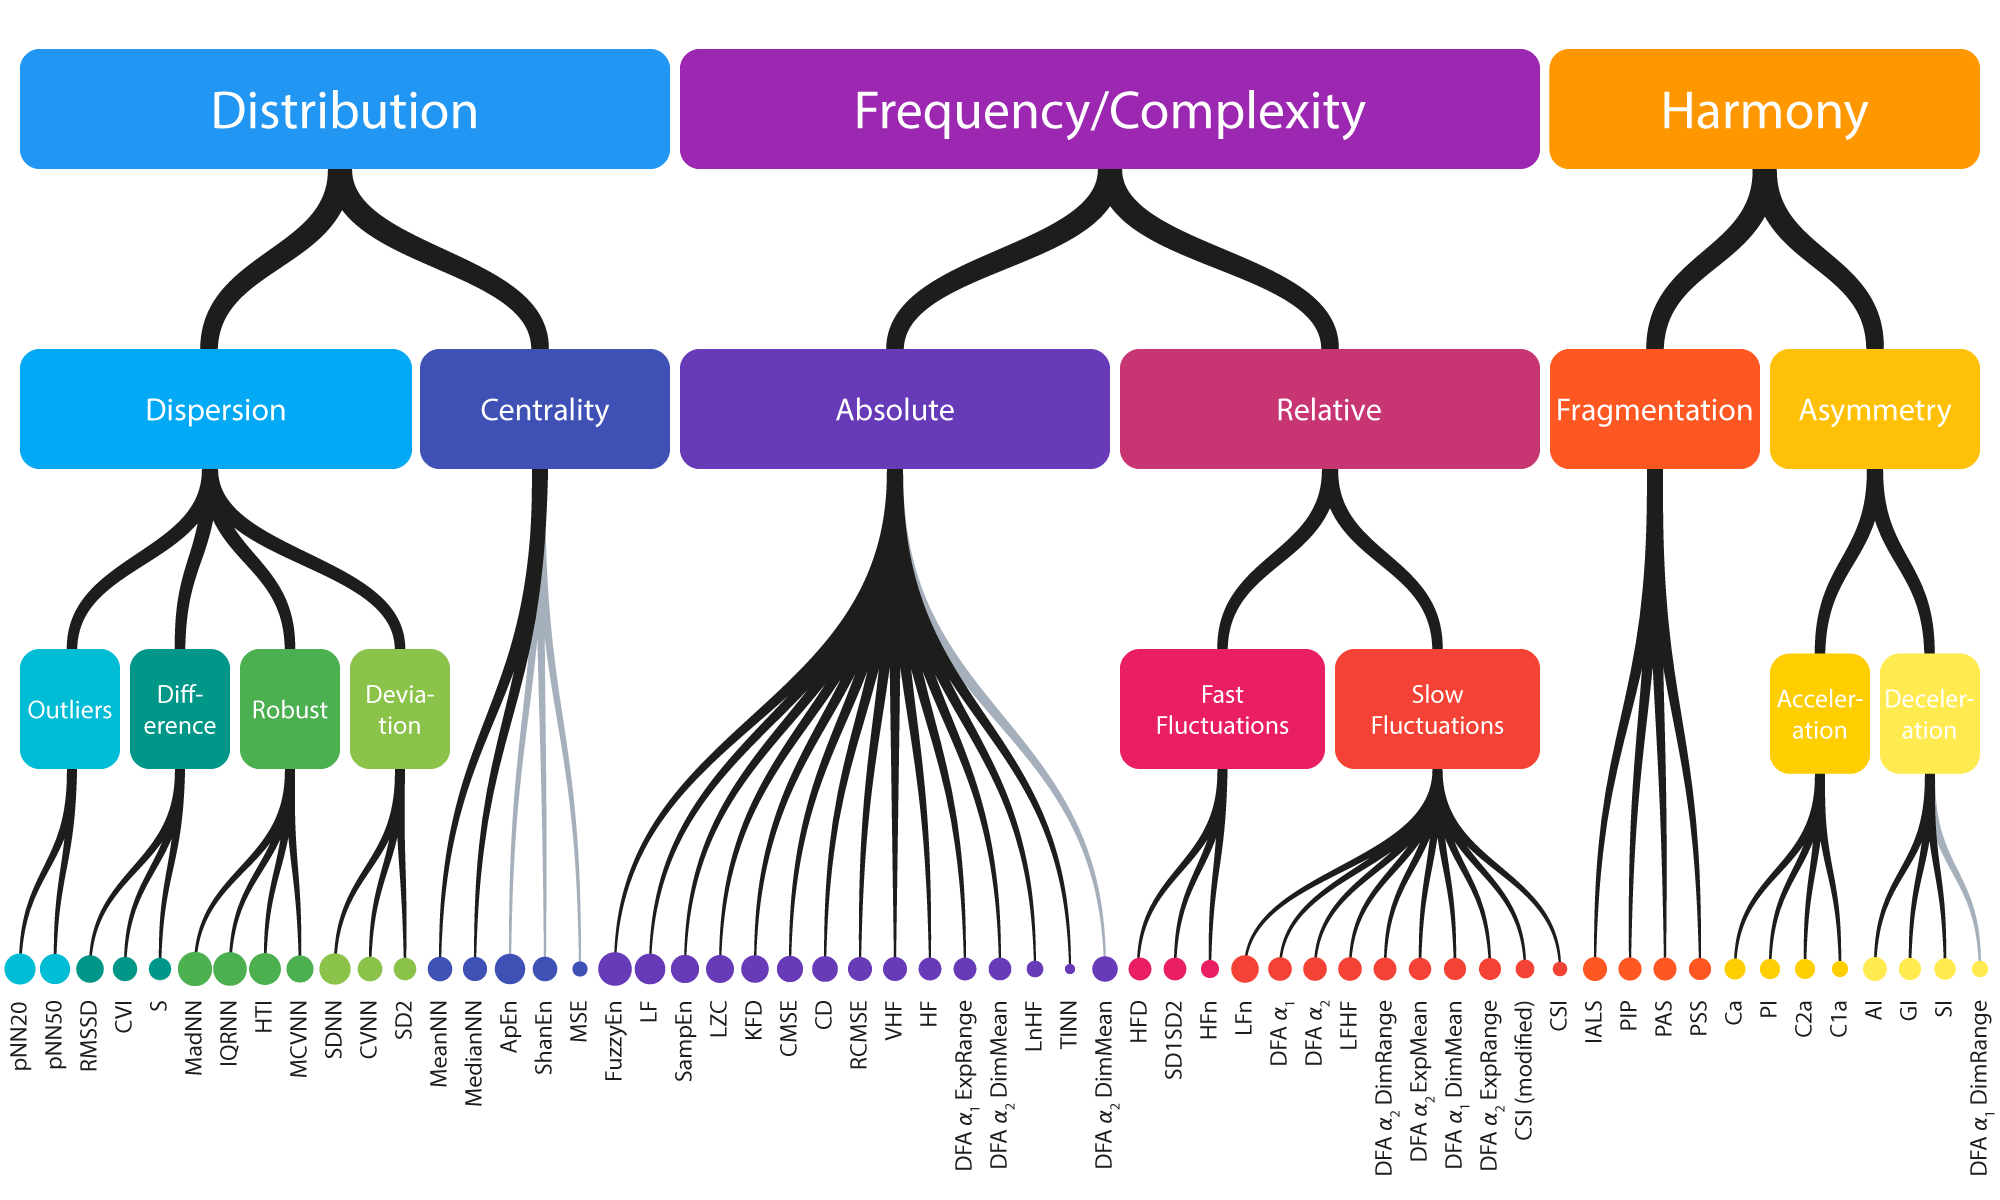
\includegraphics[width=0.5\textwidth]{figures/figure_dendrogram} 

}

\caption{Meta-Clustering Hierarchical Structure. The Level 1 clusters, determined at a vertical height cut of 0.9, include Distribution, Frequency/Complexity and Harmony. The Level 2 clusters, determined at a vertical height cut of 0.8, include Dispersion, Centrality, Absolute, Relative, Fragmentation and Asymmetry. The Level 3 clusters were only determined for groups where literature corroborates the associations between the indices. The hierarchical links are grey for associations that are less clear. The colors and the sizes of the nodes are according to their Level 2 groupings and their centrality values respectively; the bigger the nodes, the closer the indices to the cluster centres and the more representative they are of the indices' shared characteristics.}\label{fig:Figure2}
\end{figure}

The first main group, henceforth labelled as ``distribution,'' comprises predominantly time-domain indices. The groupings within this cluster suggest that it includes indices particularly sensitive to two fundamental statistical features of a variable distribution (Cardinal, 2015), namely central tendency and dispersion. One can observe the presence of a distinct sub-cluster made of \emph{MeanNN} and \emph{MedianNN}, which describes the centre of the distribution of HR. The second sub-cluster includes different mathematical descriptions of dispersion (e.g., the \emph{SD}, the \emph{IQR} or the \emph{MAD} of NN intervals). These dispersion indices are further grouped in accordance with their statistical properties and formulations. For instance, \emph{pNN20} and \emph{pNN50}, which share the same statistical origin of threshold-based variability (Kim et al., 2009), are the closest to each other. \emph{MCVNN} or \emph{MadNN} are dispersion indices that are more robust against extreme values (Pham et al., 2021), and are closer to the geometrical-based index \emph{HTI}, while \emph{CVNN}, \emph{SDNN} and \emph{SD2}, which are more sensitive to outliers (Leys et al., 2013), are in close proximity to each other. Indices that focus on the difference between successive NN intervals, such as \emph{RMSSD}, \emph{CVI} and \emph{S}, are clustered together. These groupings are consistent with the existing literature (Antink et al., 2021; Guzik et al., 2007; Malik, 1996; Pham et al., 2021; Shaffer et al., 2014). Regarding their relative importance, measured by their centrality values, \emph{MadNN}, \emph{IQRNN}, \emph{HTI}, \emph{pNN20}, and \emph{SDNN} appear to be the most representative dispersion indices. However, the difference between their centrality level is marginal (as illustrated by the size of the nodes in \textbf{Figure 2} and their centrality values in \textbf{Table 1}). Consequently, choosing to prioritize the most commonly used dispersion indices, such as \emph{SDNN} and \emph{RMSSD} (Billman, 2011) can be seen as appropriate. An alternative option would be to focus on \emph{MadNN}, \emph{pNN20}, and \emph{RMSSD}, which together offer better coverage of the fine-grained sub-groupings.

The second main group, henceforth labelled as ``harmony,'' comprises indices that are formulated to capture the abnormal properties of sinus rhythm and are sensitive to the stability of HRV. One of the two sub-clusters in this group includes only \emph{HRA} indices which measure the asymmetric contribution of HR acceleration and deceleration to HRV (Guzik et al., 2006; Piskorski \& Guzik, 2011; Yan et al., 2017). At the lower level in the hierarchical structure, depending on the asymmetric focus of the indices, the \emph{HRA} sub-cluster is further divided into two groups, namely acceleration (e.g., \emph{PI}, \emph{Ca}) or deceleration (e.g., \emph{AI}, \emph{GI}, \emph{SI}). At the higher level, this sub-cluster is joined with a distinct group of \emph{HRF} indices, which measure the ``erratic'' behaviours in heart rhythm, manifesting as abrupt and high frequency switching between the increases and decreases of HR (Costa et al., 2017, 2018). This study is the first that examined the relationships between \emph{HRA} and \emph{HRF} indices and therefore, the specific physiological mechanisms underlying their close proximity should be further investigated. Nevertheless, as existing literature has highlighted the diagnostic values of both indices, especially for cardiac disorders (Bergfeldt \& Haga, 2003; Costa et al., 2017, 2018; Costa \& Goldberger, 2019; Guzik et al., 2013; Karmakar et al., 2012; Rohila \& Sharma, 2020b), possible explanations for their close associations could stem from their ability to capture specific shared cardiac abnormalities. The centrality values of the indices in this group suggest that \emph{PI} and \emph{AI} are the most representative indices of \emph{HRA}. While there exists only a minute difference between the centrality values of \emph{HRF} indices, given that \emph{PAS} quantifies a sub-type of fragmentation that is not always accordant with the other values (Costa et al., 2017), we recommend reporting \emph{PAS} with at least another \emph{HRF} index to more comprehensively capture the nature of fragmentation.

The third high-level cluster comprises mainly frequency-domain and complexity-based HRV indices, and is henceforth descriptively labelled as ``frequency/complexity.'' The high level of similarity between \emph{DFA} and frequency-weighted spectral indices aligns with previous literature that has theoretically demonstrated and empirically verified their proximity (Captur et al., 2017; Francis et al., 2002; Lensen et al., 2020; Young \& Benton, 2015). Specifically, the \(\alpha1\) component has been shown to be particularly sensitive to the proportion of low-frequency fluctuations (e.g., \emph{LFn}, \emph{LFHF}) in the signal, and the \(\alpha2\) component to that of very-low-frequency variabilities (Captur et al., 2017; Francis et al., 2002). Nevertheless, due to the constraint of recording lengths, \emph{VLF} indices could not be properly examined in this study to verify their relationship with \(\alpha2\). The sub-cluster of \emph{DFA} and low-frequency components also includes some \emph{MF-DFA} indices such as multi-fractal dimensional ranges and dimensional means. These indices are relatively new quantifications of HRV, and thus future studies should attempt to explore them in tandem with more traditional HRV indices to better understand the underlying reason for these observed relationships. Except for three entropy-based measures - \emph{ApEn}, \emph{ShanEn} and \emph{MSE} - which seem to be more related to the centrality-based indices in the core variability features, all complexity-based indices appear to fall within this frequency-complexity cluster. To our knowledge, given the novelty of complexity-based indices in the study of HRV, only one study has examined their relationships with other HRV indices. In line with our results, Rohila and Sharma (2020a) similarly observed a strong association between frequency-based and complexity-based measures. Further investigation is thus needed to understand the origins underlying their stable associations.

A few limitations have to be underlined. Firstly, the lack of data with very long recordings limited the exploration of indices sensitive to very slow rhythms. Additionally, there were substantial discrepancies in the recording lengths of the different databases used. Although recording length can affect the quality and accuracy of several HRV indices (Chou et al., 2021), our data analysis assumed - by design - that the relationship between indices is invariant across time (i.e., that the proximity of two indices does not change for short and long recordings). Although this assumption seems mathematically justified, the alternative hypothesis remains an avenue opened for exploration. Secondly, the databases involved participants with different characteristics (in terms of health or demographic variables). Similarly, this is not an issue in and of itself, as our study was focused on the relationship between indices, rather than between (groups of) individuals. It is, however, also not impossible that the relationship between indices (and thus, the cluster structure) might marginally change in specific populations (e.g., severe heart diseases), and such speculations could be investigated in further studies. Finally, we treated each clustering approach and solution equally and assigned equal weights to the different methods in our final meta-clustering model. Future studies providing evidence that some approaches are inherently better or worse for the analysis of these physiological indices could be integrated within a meta-clustering approach by assigning different weights to different methods, based on prior knowledge, that was unfortunately not available for the current study.

In conclusion, this study aimed at describing the structure and relationships between the multitude of existing HRV indices, to provide users and readers with empirical evidence as to the latent dimensions that these indices capture, and guidelines as to which to prioritize. Indeed, given that resource-intensive efforts are needed to compute and discuss results related to every single HRV measure, most studies opt to report a few of them, often without a clear justification for their choice of indices. Such a conundrum can benefit from a greater in-depth understanding of the relationships between the HRV indices, which could, in turn, allow more informed selections of HRV indices specific to research- or clinical-oriented purposes. By recognizing the similarities and differences across these indices, groups of measures could be identified based on their ability to provide distinct information about the underlying HRV characteristics. Our work here establishes a framework that could guide the development of a more parsimonious categorization of HRV indices based on their actual level of similarity or shared physiological origins, above and beyond their mathematical origins and associations.

\hypertarget{author-contributions}{%
\section{Author Contributions}\label{author-contributions}}

DM conceived and TP coordinated the study. TP and ZL participated in the manuscript drafting. DM and AC performed a critical review of the manuscript. All authors read and approved the final manuscript.

\hypertarget{funding}{%
\section{Funding}\label{funding}}

This study was supported by the Nanyang Technological University Presidential Postdoctoral Fellowship 03INS001035C430.

\hypertarget{conflict-of-interest-statement}{%
\section{Conflict of Interest Statement}\label{conflict-of-interest-statement}}

The authors declare that the research was conducted in the absence of any commercial or financial relationships that could be construed as a potential conflict of interest.

\newpage

\hypertarget{references}{%
\section{References}\label{references}}

\begingroup
\setlength{\parindent}{-0.5in}
\setlength{\leftskip}{0.5in}

\hypertarget{refs}{}
\begin{CSLReferences}{1}{0}
\leavevmode\hypertarget{ref-acharya2006heart}{}%
Acharya, U. R., Joseph, K. P., Kannathal, N., Lim, C. M., \& Suri, J. S. (2006). Heart rate variability: A review. \emph{Medical and Biological Engineering and Computing}, \emph{44}(12), 1031--1051.

\leavevmode\hypertarget{ref-antink2021accuracy}{}%
Antink, C. H., Mai, Y., Peltokangas, M., Leonhardt, S., Oksala, N., \& Vehkaoja, A. (2021). Accuracy of heart rate variability estimated with reflective wrist-PPG in elderly vascular patients. \emph{Scientific Reports}, \emph{11}(1), 1--12.

\leavevmode\hypertarget{ref-bassett2016literature}{}%
Bassett, D. (2016). A literature review of heart rate variability in depressive and bipolar disorders. \emph{Australian \& New Zealand Journal of Psychiatry}, \emph{50}(6), 511--519.

\leavevmode\hypertarget{ref-bergfeldt2003power}{}%
Bergfeldt, L., \& Haga, Y. (2003). Power spectral and poincar{é} plot characteristics in sinus node dysfunction. \emph{Journal of Applied Physiology}, \emph{94}(6), 2217--2224.

\leavevmode\hypertarget{ref-bhattacharjee2001classification}{}%
Bhattacharjee, A., Richards, W. G., Staunton, J., Li, C., Monti, S., Vasa, P., Ladd, C., Beheshti, J., Bueno, R., Gillette, M., \& others. (2001). Classification of human lung carcinomas by mRNA expression profiling reveals distinct adenocarcinoma subclasses. \emph{Proceedings of the National Academy of Sciences}, \emph{98}(24), 13790--13795.

\leavevmode\hypertarget{ref-bigger1989comparison}{}%
Bigger Jr, J. T., Albrecht, P., Steinman, R. C., Rolnitzky, L. M., Fleiss, J. L., \& Cohen, R. J. (1989). Comparison of time-and frequency domain-based measures of cardiac parasympathetic activity in holter recordings after myocardial infarction. \emph{The American Journal of Cardiology}, \emph{64}(8), 536--538.

\leavevmode\hypertarget{ref-billman2011heart}{}%
Billman, G. E. (2011). Heart rate variability--a historical perspective. \emph{Frontiers in Physiology}, \emph{2}, 86.

\leavevmode\hypertarget{ref-brennan2001existing}{}%
Brennan, M., Palaniswami, M., \& Kamen, P. (2001). Do existing measures of poincare plot geometry reflect nonlinear features of heart rate variability? \emph{IEEE Transactions on Biomedical Engineering}, \emph{48}(11), 1342--1347.

\leavevmode\hypertarget{ref-brennan2002poincare}{}%
Brennan, M., Palaniswami, M., \& Kamen, P. (2002). Poincare plot interpretation using a physiological model of HRV based on a network of oscillators. \emph{American Journal of Physiology-Heart and Circulatory Physiology}, \emph{283}(5), H1873--H1886.

\leavevmode\hypertarget{ref-captur2017fractal}{}%
Captur, G., Karperien, A. L., Hughes, A. D., Francis, D. P., \& Moon, J. C. (2017). The fractal heart---embracing mathematics in the cardiology clinic. \emph{Nature Reviews Cardiology}, \emph{14}(1), 56--64.

\leavevmode\hypertarget{ref-cardinal2015central}{}%
Cardinal, L. J. (2015). Central tendency and variability in biological systems. \emph{Journal of Community Hospital Internal Medicine Perspectives}, \emph{5}(3), 27930.

\leavevmode\hypertarget{ref-chou2021effects}{}%
Chou, E.-F., Khine, M., Lockhart, T., \& Soangra, R. (2021). Effects of ECG data length on heart rate variability among young healthy adults. \emph{Sensors}, \emph{21}(18), 6286.

\leavevmode\hypertarget{ref-ciccone2017reminder}{}%
Ciccone, A. B., Siedlik, J. A., Wecht, J. M., Deckert, J. A., Nguyen, N. D., \& Weir, J. P. (2017). Reminder: RMSSD and SD1 are identical heart rate variability metrics. \emph{Muscle \& Nerve}, \emph{56}(4), 674--678.

\leavevmode\hypertarget{ref-costa2017heart}{}%
Costa, M. D., Davis, R. B., \& Goldberger, A. L. (2017). Heart rate fragmentation: A new approach to the analysis of cardiac interbeat interval dynamics. \emph{Frontiers in Physiology}, \emph{8}, 255.

\leavevmode\hypertarget{ref-costa2019heart}{}%
Costa, M. D., \& Goldberger, A. L. (2019). Heart rate fragmentation: Using cardiac pacemaker dynamics to probe the pace of biological aging. \emph{American Journal of Physiology-Heart and Circulatory Physiology}, \emph{316}(6), H1341--H1344.

\leavevmode\hypertarget{ref-costa2018heart}{}%
Costa, M. D., Redline, S., Davis, R. B., Heckbert, S. R., Soliman, E. Z., \& Goldberger, A. L. (2018). Heart rate fragmentation as a novel biomarker of adverse cardiovascular events: The multi-ethnic study of atherosclerosis. \emph{Frontiers in Physiology}, \emph{9}, 1117.

\leavevmode\hypertarget{ref-dormann2013collinearity}{}%
Dormann, C. F., Elith, J., Bacher, S., Buchmann, C., Carl, G., Carré, G., Marquéz, J. R. G., Gruber, B., Lafourcade, B., Leitão, P. J., \& others. (2013). Collinearity: A review of methods to deal with it and a simulation study evaluating their performance. \emph{Ecography}, \emph{36}(1), 27--46.

\leavevmode\hypertarget{ref-fatisson2016influence}{}%
Fatisson, J., Oswald, V., \& Lalonde, F. (2016). Influence diagram of physiological and environmental factors affecting heart rate variability: An extended literature overview. \emph{Heart International}, \emph{11}(1), heartint--5000232.

\leavevmode\hypertarget{ref-faust2004analysis}{}%
Faust, O., Acharya, R., Krishnan, S., \& Min, L. C. (2004). Analysis of cardiac signals using spatial filling index and time-frequency domain. \emph{BioMedical Engineering OnLine}, \emph{3}(1), 1--11.

\leavevmode\hypertarget{ref-forte2019heart}{}%
Forte, G., Favieri, F., \& Casagrande, M. (2019). Heart rate variability and cognitive function: A systematic review. \emph{Frontiers in Neuroscience}, \emph{13}, 710.

\leavevmode\hypertarget{ref-francis2002physiological}{}%
Francis, D. P., Willson, K., Georgiadou, P., Wensel, R., Davies, L. C., Coats, A., \& Piepoli, M. (2002). Physiological basis of fractal complexity properties of heart rate variability in man. \emph{The Journal of Physiology}, \emph{542}(2), 619--629.

\leavevmode\hypertarget{ref-golberger1996non}{}%
Golberger, A. (1996). Non-linear dynamics for clinicians: Chaos theory, fractals, and complexity at the bedside. \emph{The Lancet}, \emph{347}(9011), 1312--1314.

\leavevmode\hypertarget{ref-goldberger2000physiobank}{}%
Goldberger, A. L., Amaral, L. A., Glass, L., Hausdorff, J. M., Ivanov, P. C., Mark, R. G., Mietus, J. E., Moody, G. B., Peng, C.-K., \& Stanley, H. E. (2000). PhysioBank, PhysioToolkit, and PhysioNet: Components of a new research resource for complex physiologic signals. \emph{Circulation}, \emph{101}(23), e215--e220.

\leavevmode\hypertarget{ref-Golino_2017}{}%
Golino, H. F., \& Epskamp, S. (2017). Exploratory graph analysis: A new approach for estimating the number of dimensions in psychological research. \emph{{PLOS} {ONE}}, \emph{12}(6), e0174035. \url{https://doi.org/10.1371/journal.pone.0174035}

\leavevmode\hypertarget{ref-Golino_2020}{}%
Golino, H., Shi, D., Christensen, A. P., Garrido, L. E., Nieto, M. D., Sadana, R., Thiyagarajan, J. A., \& Martinez-Molina, A. (2020). Investigating the performance of exploratory graph analysis and traditional techniques to identify the number of latent factors: A simulation and tutorial. \emph{Psychological Methods}, \emph{25}(3), 292--320. \url{https://doi.org/10.1037/met0000255}

\leavevmode\hypertarget{ref-guzik2013obstructive}{}%
Guzik, P., Piskorski, J., Awan, K., Krauze, T., Fitzpatrick, M., \& Baranchuk, A. (2013). Obstructive sleep apnea and heart rate asymmetry microstructure during sleep. \emph{Clinical Autonomic Research}, \emph{23}(2), 91--100.

\leavevmode\hypertarget{ref-guzik2007correlations}{}%
Guzik, P., Piskorski, J., Krauze, T., Schneider, R., Wesseling, K. H., Wykretowicz, A., \& Wysocki, H. (2007). Correlations between poincare plot and conventional heart rate variability parameters assessed during paced breathing. \emph{The Journal of Physiological Sciences}, 0702020009--0702020009.

\leavevmode\hypertarget{ref-guzik2006heart}{}%
Guzik, P., Piskorski, J., Krauze, T., Wykretowicz, A., \& Wysocki, H. (2006). \emph{Heart rate asymmetry by poincar{é} plots of RR intervals}.

\leavevmode\hypertarget{ref-hayano2019pitfalls}{}%
Hayano, J., \& Yuda, E. (2019). Pitfalls of assessment of autonomic function by heart rate variability. \emph{Journal of Physiological Anthropology}, \emph{38}(1), 1--8.

\leavevmode\hypertarget{ref-hennig2015package}{}%
Hennig, C., \& Imports, M. (2015). Package {`fpc.'} \emph{Flexible Procedures for Clustering}.

\leavevmode\hypertarget{ref-howell2018high}{}%
Howell, L., \& Porr, B. (2018). \emph{High precision ecg database with annotated r peaks, recorded and filmed under realistic conditions}.

\leavevmode\hypertarget{ref-iyengar1996age}{}%
Iyengar, N., Peng, C., Morin, R., Goldberger, A. L., \& Lipsitz, L. A. (1996). Age-related alterations in the fractal scaling of cardiac interbeat interval dynamics. \emph{American Journal of Physiology-Regulatory, Integrative and Comparative Physiology}, \emph{271}(4), R1078--R1084.

\leavevmode\hypertarget{ref-karmakar2012investigating}{}%
Karmakar, C., Khandoker, A., \& Palaniswami, M. (2012). Investigating the changes in heart rate asymmetry (HRA) with perturbation of parasympathetic nervous system. \emph{Australasian Physical \& Engineering Sciences in Medicine}, \emph{35}(4), 465--474.

\leavevmode\hypertarget{ref-kim2009pnnx}{}%
Kim, J.-H., Yi, S. H., Ahn, Y. M., Lee, K. Y., Yang, S. A., \& Kim, Y. S. (2009). The pNNx heart rate variability statistics: An application to neuroautonomic dysfunction of clozapine-treated subjects. \emph{Psychiatry Investigation}, \emph{6}(4), 294.

\leavevmode\hypertarget{ref-kleiger2005heart}{}%
Kleiger, R. E., Stein, P. K., \& Bigger Jr, J. T. (2005). Heart rate variability: Measurement and clinical utility. \emph{Annals of Noninvasive Electrocardiology}, \emph{10}(1), 88--101.

\leavevmode\hypertarget{ref-kudat2006heart}{}%
Kudat, H., Akkaya, V., Sozen, A., Salman, S., Demirel, S., Ozcan, M., Atilgan, D., Yilmaz, M., \& Guven, O. (2006). Heart rate variability in diabetes patients. \emph{Journal of International Medical Research}, \emph{34}(3), 291--296.

\leavevmode\hypertarget{ref-kuncheva2014combining}{}%
Kuncheva, L. I. (2014). \emph{Combining pattern classifiers: Methods and algorithms}. John Wiley \& Sons.

\leavevmode\hypertarget{ref-laitio2007role}{}%
Laitio, T., Jalonen, J., Kuusela, T., \& Scheinin, H. (2007). The role of heart rate variability in risk stratification for adverse postoperative cardiac events. \emph{Anesthesia \& Analgesia}, \emph{105}(6), 1548--1560.

\leavevmode\hypertarget{ref-lau2021brain}{}%
Lau, Z. J., Pham, T., Chen, S. A., \& Makowski, D. (2021). \emph{Brain entropy, fractal dimensions and predictability: A review of complexity measures for EEG in healthy and neuropsychiatric populations}.

\leavevmode\hypertarget{ref-leite2015correlation}{}%
Leite, M. R., Ramos, E. M. C., Kalva-Filho, C. A., Rodrigues, F. M. M., Freire, A. P. C., Tacao, G. Y., Toledo, A. C. de, Cecilio, M. J., Vanderlei, L. C. M., \& Ramos, D. (2015). Correlation between heart rate variability indexes and aerobic physiological variables in patients with COPD. \emph{Respirology}, \emph{20}(2), 273--278.

\leavevmode\hypertarget{ref-lensen2020heart}{}%
Lensen, I. S., Monfredi, O. J., Andris, R. T., Lake, D. E., \& Moorman, J. R. (2020). Heart rate fragmentation gives novel insights into non-autonomic mechanisms governing beat-to-beat control of the heart's rhythm. \emph{JRSM Cardiovascular Disease}, \emph{9}, 2048004020948732.

\leavevmode\hypertarget{ref-leys2013detecting}{}%
Leys, C., Ley, C., Klein, O., Bernard, P., \& Licata, L. (2013). Detecting outliers: Do not use standard deviation around the mean, use absolute deviation around the median. \emph{Journal of Experimental Social Psychology}, \emph{49}(4), 764--766.

\leavevmode\hypertarget{ref-ludecke2019insight}{}%
Ludecke, D., Waggoner, P. D., \& Makowski, D. (2019). Insight: A unified interface to access information from model objects in r. \emph{Journal of Open Source Software}, \emph{4}(38), 1412.

\leavevmode\hypertarget{ref-ludecke2020extracting}{}%
Lüdecke, D., Ben-Shachar, M. S., Patil, I., \& Makowski, D. (2020). Extracting, computing and exploring the parameters of statistical models using r. \emph{Journal of Open Source Software}, \emph{5}(53), 2445.

\leavevmode\hypertarget{ref-ludecke2021performance}{}%
Lüdecke, D., Ben-Shachar, M. S., Patil, I., Waggoner, P., \& Makowski, D. (2021). Performance: An r package for assessment, comparison and testing of statistical models. \emph{Journal of Open Source Software}, \emph{6}(60).

\leavevmode\hypertarget{ref-ludecke2021see}{}%
Lüdecke, D., Patil, I., Ben-Shachar, M. S., Wiernik, B. M., Waggoner, P., \& Makowski, D. (2021). See: An r package for visualizing statistical models. \emph{Journal of Open Source Software}, \emph{6}(64), 3393.

\leavevmode\hypertarget{ref-makowski2019bayestestr}{}%
Makowski, D., Ben-Shachar, M. S., \& Ludecke, D. (2019). bayestestR: Describing effects and their uncertainty, existence and significance within the bayesian framework. \emph{Journal of Open Source Software}, \emph{4}(40), 1541.

\leavevmode\hypertarget{ref-makowski2020methods}{}%
Makowski, D., Ben-Shachar, M. S., Patil, I., \& Lüdecke, D. (2020). Methods and algorithms for correlation analysis in r. \emph{Journal of Open Source Software}, \emph{5}(51), 2306.

\leavevmode\hypertarget{ref-makowski2021neurokit2}{}%
Makowski, D., Pham, T., Lau, Z. J., Brammer, J. C., Lespinasse, F., Pham, H., Schölzel, C., \& Chen, S. A. (2021). NeuroKit2: A python toolbox for neurophysiological signal processing. \emph{Behavior Research Methods}, 1--8.

\leavevmode\hypertarget{ref-malik1996heart}{}%
Malik, M. (1996). Heart rate variability: Standards of measurement, physiological interpretation, and clinical use: Task force of the european society of cardiology and the north american society for pacing and electrophysiology. \emph{Annals of Noninvasive Electrocardiology}, \emph{1}(2), 151--181.

\leavevmode\hypertarget{ref-mela2002impact}{}%
Mela, C. F., \& Kopalle, P. K. (2002). The impact of collinearity on regression analysis: The asymmetric effect of negative and positive correlations. \emph{Applied Economics}, \emph{34}(6), 667--677.

\leavevmode\hypertarget{ref-monti2003consensus}{}%
Monti, S., Tamayo, P., Mesirov, J., \& Golub, T. (2003). Consensus clustering: A resampling-based method for class discovery and visualization of gene expression microarray data. \emph{Machine Learning}, \emph{52}(1), 91--118.

\leavevmode\hypertarget{ref-moody2001impact}{}%
Moody, G. B., \& Mark, R. G. (2001). The impact of the MIT-BIH arrhythmia database. \emph{IEEE Engineering in Medicine and Biology Magazine}, \emph{20}(3), 45--50.

\leavevmode\hypertarget{ref-nguyen2019improving}{}%
Nguyen Phuc Thu, T., Hernandez, A. I., Costet, N., Patural, H., Pichot, V., Carrault, G., \& Beuchee, A. (2019). Improving methodology in heart rate variability analysis for the premature infants: Impact of the time length. \emph{PloS One}, \emph{14}(8), e0220692.

\leavevmode\hypertarget{ref-naes2001understanding}{}%
Næs, T., \& Mevik, B.-H. (2001). Understanding the collinearity problem in regression and discriminant analysis. \emph{Journal of Chemometrics: A Journal of the Chemometrics Society}, \emph{15}(4), 413--426.

\leavevmode\hypertarget{ref-otzenberger1998dynamic}{}%
Otzenberger, H., Gronfier, C., Simon, C., Charloux, A., Ehrhart, J., Piquard, F., \& Brandenberger, G. (1998). Dynamic heart rate variability: A tool for exploring sympathovagal balance continuously during sleep in men. \emph{American Journal of Physiology-Heart and Circulatory Physiology}, \emph{275}(3), H946--H950.

\leavevmode\hypertarget{ref-peng2015extraction}{}%
Peng, R.-C., Zhou, X.-L., Lin, W.-H., \& Zhang, Y.-T. (2015). Extraction of heart rate variability from smartphone photoplethysmograms. \emph{Computational and Mathematical Methods in Medicine}, \emph{2015}.

\leavevmode\hypertarget{ref-pham2021heart}{}%
Pham, T., Lau, Z. J., Chen, S., \& Makowski, D. (2021). Heart rate variability in psychology: A review of HRV indices and an analysis tutorial. \emph{Sensors}, \emph{21}(12), 3998.

\leavevmode\hypertarget{ref-piskorski2011asymmetric}{}%
Piskorski, J., \& Guzik, P. (2011). Asymmetric properties of long-term and total heart rate variability. \emph{Medical \& Biological Engineering \& Computing}, \emph{49}(11), 1289--1297.

\leavevmode\hypertarget{ref-R-base}{}%
R Core Team. (2019). \emph{R: A language and environment for statistical computing}. R Foundation for Statistical Computing. \url{https://www.R-project.org/}

\leavevmode\hypertarget{ref-rohila2020correlation}{}%
Rohila, A., \& Sharma, A. (2020a). Correlation between heart rate variability features. \emph{2020 7th International Conference on Signal Processing and Integrated Networks (SPIN)}, 669--674.

\leavevmode\hypertarget{ref-rohila2020asymmetric}{}%
Rohila, A., \& Sharma, A. (2020b). Asymmetric spread of heart rate variability. \emph{Biomedical Signal Processing and Control}, \emph{60}, 101985.

\leavevmode\hypertarget{ref-rossi2015impact}{}%
Rossi, R. C., Vanderlei, L. C. M., Goncalves, A. C. C. R., Vanderlei, F. M., Bernardo, A. F. B., Yamada, K. M. H., Silva, N. T. da, \& Abreu, L. C. de. (2015). Impact of obesity on autonomic modulation, heart rate and blood pressure in obese young people. \emph{Autonomic Neuroscience}, \emph{193}, 138--141.

\leavevmode\hypertarget{ref-shaffer2014healthy}{}%
Shaffer, F., McCraty, R., \& Zerr, C. L. (2014). A healthy heart is not a metronome: An integrative review of the heart's anatomy and heart rate variability. \emph{Frontiers in Psychology}, \emph{5}, 1040.

\leavevmode\hypertarget{ref-suzuki2006pvclust}{}%
Suzuki, R., \& Shimodaira, H. (2006). Pvclust: An r package for assessing the uncertainty in hierarchical clustering. \emph{Bioinformatics}, \emph{22}(12), 1540--1542.

\leavevmode\hypertarget{ref-voss2009methods}{}%
Voss, A., Schulz, S., Schroeder, R., Baumert, M., \& Caminal, P. (2009). Methods derived from nonlinear dynamics for analysing heart rate variability. \emph{Philosophical Transactions of the Royal Society A: Mathematical, Physical and Engineering Sciences}, \emph{367}(1887), 277--296.

\leavevmode\hypertarget{ref-yan2017area}{}%
Yan, C., Li, P., Ji, L., Yao, L., Karmakar, C., \& Liu, C. (2017). Area asymmetry of heart rate variability signal. \emph{Biomedical Engineering Online}, \emph{16}(1), 1--14.

\leavevmode\hypertarget{ref-young2015we}{}%
Young, H., \& Benton, D. (2015). We should be using nonlinear indices when relating heart-rate dynamics to cognition and mood. \emph{Scientific Reports}, \emph{5}(1), 1--16.

\end{CSLReferences}

\endgroup


\end{document}
